\section{Results}\label{sec:results}

\begin{figure*}
    \centering
    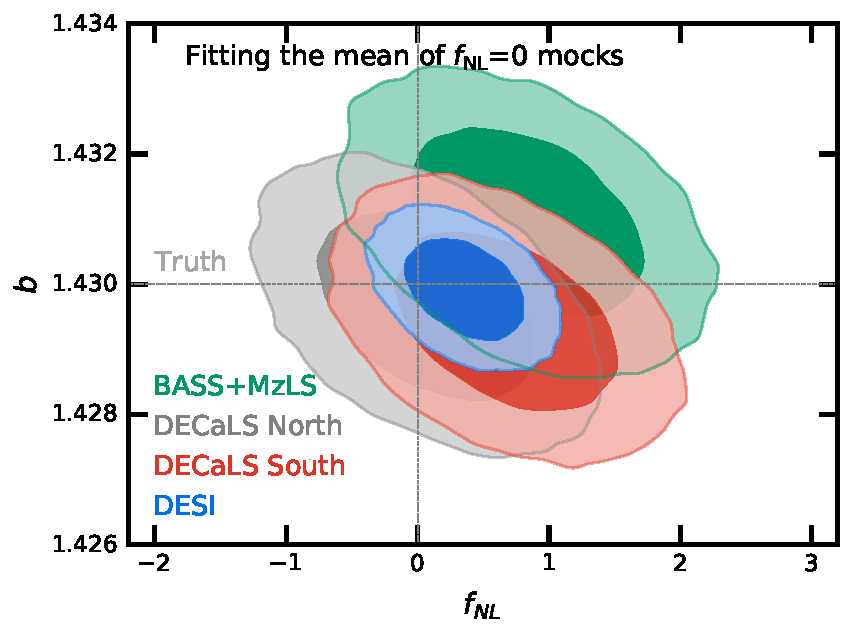
\includegraphics[width=0.45\textwidth]{figures/mcmc_zero.pdf} 
    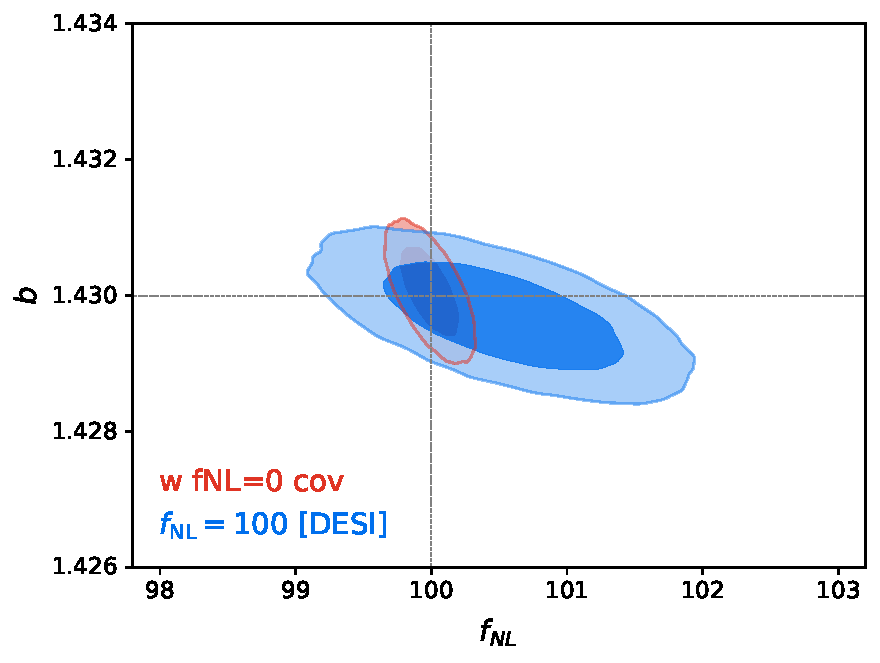
\includegraphics[width=0.45\textwidth]{figures/mcmc_po100.pdf} 
    \caption{Mock test}\label{fig:mcmc_mocks}
\end{figure*}


\begin{table*}
  \begin{center}
    \caption{Best fit and marginalized  stats for $\fnl$.}
    \label{tab:mocksmcmc}
    \begin{tabular}{lcccccc}
    \hline
    \hline
    & MAP [scipy] & MAP [chain]  &	Mean [chain]	& Median [chain] &	16th	& 84th \\
    \hline
    $\fnl$ = 0	& 0.747050	& 0.745692	& 0.739923	& 0.738965	& 0.326864	& 1.154931 \\
    $\fnl$ = 100	& 100.853749	& 100.857356	& 100.856818	& 100.857763	& 100.306626	& 101.406558
    \end{tabular}
  \end{center}
\end{table*}



\begin{figure*}
    \centering
    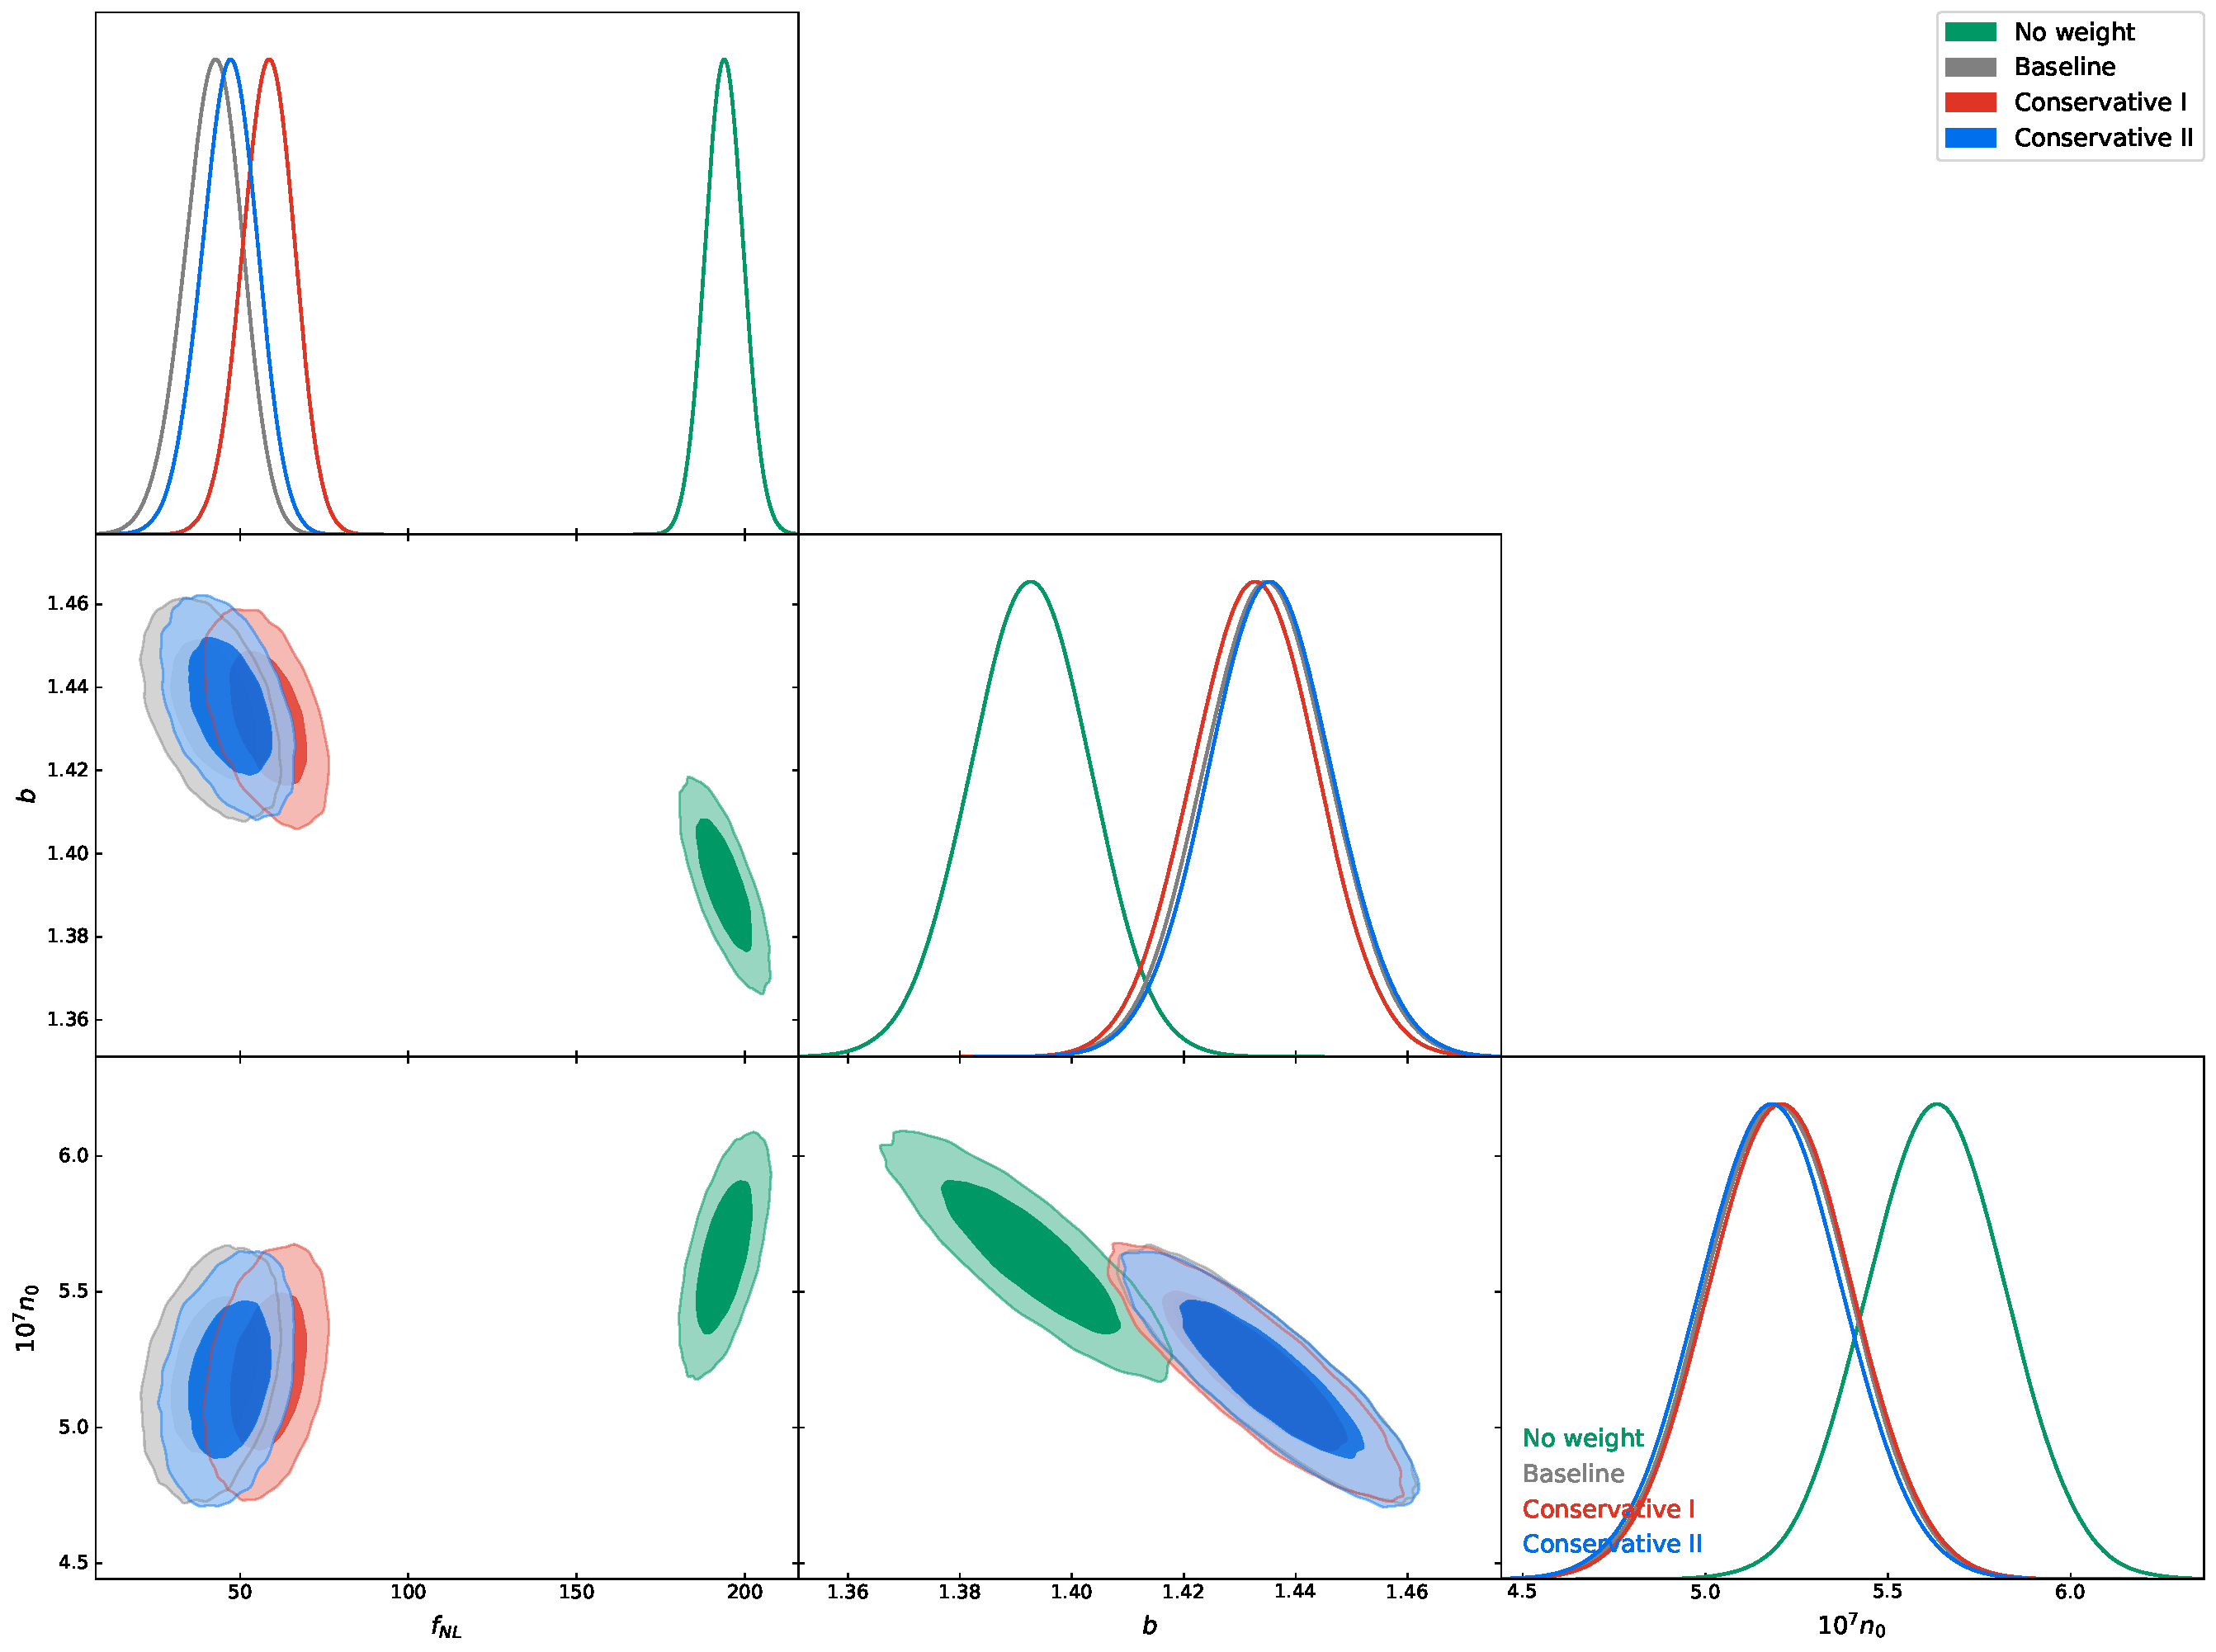
\includegraphics[width=0.95\textwidth]{figures/mcmc_dr9.pdf} 
    \caption{DR9}\label{fig:mcmc_dr9}
\end{figure*}

\begin{table*}
  \begin{center}
    \caption{Best fit and marginalized  stats for $\fnl$.}
    \label{tab:mocksmcmc}
    \begin{tabular}{lcccccc}
    \hline
    \hline
    & MAP [scipy] & MAP [chain]  &	Mean [chain]	& Median [chain] &	16th	& 84th \\
    \hline
No Weight	 & 193.799114 &	193.834016	& 193.896075 &	193.867594&	188.480955&	199.329321 \\
Baseline&	42.555440&	42.442136&	41.954523&	42.221369&	33.689653&	50.194945\\
Conservative I &	58.635294 &	58.900166&	58.279580&	58.432779&	50.853873&	65.686198 \\
Conservative II	& 47.556331 &	47.567315 &	46.739960 &	46.920699 &	38.736039 &	54.729885 
    \end{tabular}
  \end{center}
\end{table*}

%	

%fNL = 100	100.853749	100.857356	100.856818	100.857763	100.306626	101.406558
